\chapter{Implementation of RoboMission}
\label{chap:implementation-of-robomission}

This chapter describes general architecture of the RoboMission application,
together with a few specific aspects, such as representation of task sources,
and transformation between programming blocks and code.

\section{System Architecture}

The application uses a client-server architecture,
with a fat frontend client communicating with the server backend via REST API.
In addition to the frontend app and backend service,
there are two other parts of the system:
scheduled jobs, which run periodically every night (e.g. metrics computation),
and tools for offline analysis of collected data
(e.g. jupyter notebooks). % templates).
% TODO: and "helper functions"
% TODO: ref/cite human-in-the-loop principle
% TODO: consider: list the parts in itemize
% TODO: other potential parts (future):
% - tasks/content management tools (CLI+browser)
% - simulations (CLI+browser)
% TODO: consider to include FE and BE sections below as subsections of this section
%TODO: diagram of overall architecture (client-server, communication, monitoring, scheduled jobs, offline analysis)

% \section{Frontend}
Frontend is a single page application with \emph{redux architecture} (CITE),
which means that a single immutable state stores all application data.
The state cannot be mutated directly; a new state can be created only
%from the old one
by dispatching actions.
Each part of the state then defines its \emph{reducer},
which is a pure function that takes previous state and action, and returns a new state.
% ... and the only way the state can be changed is by dispatching actions.
% ... dispatcher then takes dispatched actions one by one and reduce them (notifying
%     connected containers about the new state)
% ... reducers: state, action -> new state (pure functions)
% "unidirectional UI" (as opposed to MVC and similar architectures)
The view is then assembled using declarative reusable components, that can
be either \emph{presentational} (e.g. describing how the game world should be
rendered), or \emph{behavioral}, selecting data from the state to use for
the rendering, and defining actions to dispatch and their triggers.
The application also defines a few asynchronous workflows called \emph{sagas},
e.g. for program interpretation, for task solving proces, or for sending events to
Google Analytics.  % better examples?
%% TODO: at least one sentence about React components?
%\subsection{React Components}
%
%\begin{itemize}
%\item mostly declarative - simple mental model: rebuilding from scratch every time anything change -> less error prone
%\item reusability -> use of single component on many places in different contexts,

%% TODO: Improve the diagram to make a point; otherwise remove.
%\imgW{frontend-dependencies}{%
%  Frontend modules/packages and dependencies between them.}
% TODO: Give examples of (in description) of what are submodules inside core, utils, reducers, sagas, containers, components.
% TODO: Note that some dependencies are eliminated via dependency injection in
  % redux-architecture (+ example!)
% TODO: Improve diagram, use a standard notation (see slides from Software Engineering)
% TODO: Explain the difference between component and containers.

%TODO: redux-architecture (data+events flow) diagram (specifically for our app) (and show how the flow of events is easier to reason about in React+Redux (than in Angular)).

%% TODO: at least one sentence about React components?
%\subsection{React Components}
%
%\begin{itemize}
%\item mostly declarative - simple mental model: rebuilding from scratch every time anything change -> less error prone
%\item reusability -> use of single component on many places in different contexts,
%  or even outside the app (use space-world for ai-search-workshop)
%\item example from our codebase (code, image)
%\end{itemize}

% TODO: This might be relevant if shown for code interpretation instead of
% sending feedback.
%\subsection{Asynchronous Side Effects}
%\label{sec:robomission-asynchronous-side-effects}
%
%Frontend applications are usually full of asynchronous side effects
%(e.g. fetching data from server, wating for user actions).
%Many ways to handle them were proposed,
%such as callbacks (REF) or promises (REF).
%%The most basic one are callbacks --
%%asychronous function takes a function (``callback'') as a parameter
%%and calls it once the asynchronous action is resolved.
%%(TODO: mention/explain promises -- advantage: very explicit; clean error
%%handling; show example for data fetching)
%
%However, both callbacks and promises become awkward for expressing complex
%asynchronous flows, such as visualizing code execution,
%leading to unreadable ``callback hell''. % TODO: ref for callback hell
%Sagas provide an alternative way of handling asynchronous effects using generators.
%Instead of performing asynchronous effects directly, sagas yield
%descriptions of such effects.
%As an example, there is a saga responsible for processing
%submitted feedback.
%Note that while the code contains many asynchronous effects,
%it can be read nearly as easy as standard linear synchronous code.
%
%% TODO: insert comments in the code
%% TODO: mention other advantage of sagas - great testability
%% TODO: also mention new async-await concept
%
%\begin{lstlisting}[language=ES6]
%// Generator for a single submit-feedback request
%function* submitFeedback(action) {
%  const { text, email } = action.payload;
%  // Asynchronous request to get a value from state
%  const url = yield select(getFeedbackUrl);
%  try {
%    // Asynchronous request to post data to server
%    yield call(api.sendFeedback, url, text, email);
%    // Asynchronous request to dispatch a new action
%    yield put(actions.submitFeedback.success());
%  }
%  catch (error) {
%    const { fieldErrors } = error;
%    yield put(
%      actions.submitFeedback.failure(fieldErrors));
%  }
%}
%\end{lstlisting}

% TODO: add code samples for each concept (react component + image, reducer, saga)
% TODO(optional): awesome ES6 (example from our code)
% TODO(Material Design): example of our component + code

% \section{Backend}

%\begin{itemize}
%\item Django, Django Rest Framework
%\item django apps (python packages): learn, monitoring (potential diagram for planned architecture: users, tasks, learn, adaptability, monitoring, simulations, analysis)
%\item models (...), serializers, views, services/use cases/core
%\item data export
%\item monitoring app, metrics computation
%\item generators (e.g. metric computation)
%\item architecture (of individual apps): viewsets/management, services,
%serializers, models, core (actions, credits, recommendation)
%\end{itemize}

Backend is decomposed into modules defining database entities,
their serializers (JSON for sending to frontend and CSV for exports),
\emph{ViewSets} (CITE) describing REST API,
and core modules with pure functions
for computing performance, skills, and recommendation.
% TODO: + domain parsing, monitoring.
%Technologies are becoming obsolete soon,
%so will not discuss them in the text.
An overview of technologies used currently in the project
is included in \cref{chap:technologies}.


\section{Task Sources}

Each task is described by a single file in a restricted markdown format,
containing name, category, setting and solution.
The high-level grammar for task description looks like this:

\begin{lstlisting}
# <name>
[- option: value]*

## Setting
```
<SpaceWorld>
```
[- option: value]*

## Solution
```
<RoboCode>
```
\end{lstlisting}

Currently, there is one mandatory top-level option (task category)
and two optional setting options (length, energy).
(TBA: ref to example below; ref to 2 subparts - SpaceWorld grammar, RoboCode grammar)
% [consider] Markdown files are then parsed and loaded into DB by a single command.

Task sources in markdown have several advantages:
it is human readable,
each change is version-controlled,
and the task can be edited easily in any text editor.
However, it is more convenient to use online task editor (REF to task editor fig),
unless it is a really minor modification, or unless one wants to change multiple tasks at once.

% [consider]
% - Localized task names are not part of the task source,
% because all localized messages live on the same place in a single file on FE.
% - PEG grammar for parsing
% - internal represenation (DB model and its serializers for FE and for CSV exports)


Example of complete task source (for rendered task see figure \ref{fig:robomission-task1}. TBA: show rendered task and its source side by side)

\begin{lstlisting}
# turning-left
- category: moves

## Setting

```
|bM|b |b |bM|b |
|kA|k |kM|k |kA|
|k |k |kA|kM|k |
|kM|k |kS|k |kA|
```

## Solution

```
left()
fly()
fly()
```
\end{lstlisting}


% \subsection{SpaceWorld Descriptions}

Each SpaceWorld is described by a simple human-readable string.
See figure \ref{fig:spaceworld-in-editor} for an example and descripton.
Set of valid SpaceWorld descriptions can be described by the
following context-free grammar:

\begin{lstlisting}
SpaceWorld -> Row+
Row -> '|'(Field'|')+ EOL  // EOL = End Of Line
Field -> Background Object*
Background -> 'r' | 'g' | 'b' | 'y' | 'k'
Object -> 'S' | 'A' | 'M' | 'D' | 'W'
\end{lstlisting}


%\begin{figure}[h]
%\begin{center}
%\begin{subfigure}{.4\textwidth}
%\centering
%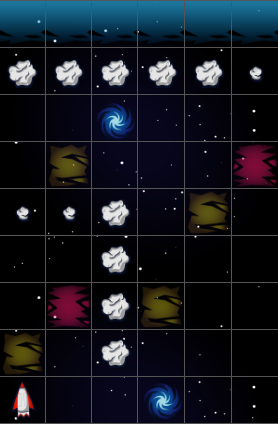
\includegraphics[width=.9\textwidth]{img/spaceworld}
%\end{subfigure}
%\begin{subfigure}{.36\textwidth}
%\centering
%{\lstset{numbers=none}
%\begin{lstlisting}
%|b |b |b |b |b |b |
%|kA|kA|kA|kA|kA|kM|
%|k |k |kW|k |k |k |
%|k |y |k |k |k |r |
%|kM|kM|kA|k |y |k |
%|k |k |kA|k |k |k |
%|k |r |kA|y |k |k |
%|y |k |kA|k |k |k |
%|kS|k |k |kW|k |k |
%\end{lstlisting}}
%\end{subfigure}
%\end{center}
%\caption{Example of Space World with its source code. TODO: Describe letters; consider replacing code listing with a screenshot from task editor with code highlighting}
%\label{fig:spaceworld-source}
%\end{figure}


\imgW[0.9]{spaceworld-in-editor}%
{Example SpaceWorld with its source code.
Each line describes one row of the grid
and is split by pipes (``|'') into fields.
Each field starts with a lower-cased letter denoting color of the field
(b -- blue, r -- red, k -- black, etc.),
followed by an optional upper-case letter denoting an object
(A -- asteroid, M -- meteoroid, W -- wormhole, S -- spaceship, etc.).
For example ``rD'' is a red field with a diamond.}



\section{RoboCode}

RoboCode is a language based on Python that is used in task sources for solutions.
It is also meant to be used in more advanced levels as the transitional phase
from block-based to text-based programming.
The requirements for the language are following:
\begin{itemize}
\item easy for beginners, understandable without previous knowledge,
\item conciseness (short, but readable programs),
\item matching Blockly blocks closely (for easy transition from Blockly),
\item matching Python closely (for easy transition to Python).
\end{itemize}

\subsection{Syntax and Semantic}
\label{sec:syntax-semantic}

% TODO[consider] note on mixing lexer+parser+some semantic analysis
% (which is partially convenient, partially confusing)

There are four commands for performing actions:
\begin{lstlisting}
fly()
left()
right()
shoot()
\end{lstlisting}
Each action is combined with moving one row forward.
The movement takes place after the action, with the exception of left and right turning actions, where the movement and the action happen simultaneously,
i.e. the spaceship flies diagonally to the left or to the right.
% TODO: Rephrase. Is confusing, because the general statement ("movement takes
% place after the action") is only relevant for shoot(), and all the other
% commands are special cases.

Loops and conditional statements are same as in the Python,
with the notable exception of the repeat loop,
which was simplified to the form matching a corresponding
Blockly block, which is easier to understand by beginners:
% TODO: ass robocode highlighting
\begin{lstlisting}
repeat 4:
    fly()
\end{lstlisting}

Tests inside while-loops and if-statements are limited to the following forms
(again in order to match the respective Blockly blocks):
\begin{lstlisting}
position() [==|!=|>|<|>=|<=] [1..6]
color() [==|!=] ['r'|'g'|'b'|'y'|'k']
<test> [and|or] <test>
\end{lstlisting}
The letters in the color-test have the same meaning as in the space world description,
('r' for red, 'g' for green, etc.)


\begin{figure}[h]
\begin{lstlisting}
while color() != 'b':
    if position() == 1:
        right()
    if position() >= 4:
        shoot()
    fly()
\end{lstlisting}
\caption{Example of a complete RoboCode program}
\label{fig:robocode-example}
\end{figure}


\subsection{RoboAST}

\begin{table}[h]
\begin{center}
\begin{tabular}{l l l}
\toprule
Name & Form & Usage  \\
\midrule
RoboCode     & textual (Python-like) & sample solutions in task sources  \\
MiniRoboCode & compact string & logging, storing in DB, analysis  \\
RoboBlocks   & Blockly blocks & code editor for students  \\
RoboJS       & textual (JavaScript) & interpretation in browser  \\
RoboAST      & json (AST) & common intermediate representation \\
\bottomrule
\end{tabular}
\end{center}
\caption{Different code representaions used within the system.}
\label{tbl:code-representation}
\end{table}

While Python-like RoboCode is convenient for writing sample solutions,
more comact form would be useful for logging, storing in DB and analysis.
Furthermore, we want a visual blocks presentation of the code for students.
Last but not least, a JavaScript equivalent of the code is needed for
interpreting the code in the browser.
(Table \ref{tbl:code-representation} shows overview of all representations.)

To avoid implementing separate transformations between each pair of these
presentations, we introduced a common intermediate representation,
\emph{RoboAST}, which is a simple Abstract Syntaxt Tree in json.
(See example of a RoboAST in figure \ref{fig:robocode-transformations-example}.)
For each supported presenation it is enough to implement
its parser returning RoboAST object, and
its generator from RoboAST (figure \ref{fig:robocode-transformations}).
With one parser and one generator for each presentation,
it is possible to transform presentation A
into presentaion B by parsing A into RoboAST and
then generating B from this RoboAST.
This mechanism also allows for switching between RoboCode and RoboBlocks
anytime during writing a solution in the task editor.
% TODO: mention the disadvantage - not able to use functionality provided by Blockly (code generators)

\imgW[0.8]{robocode-transformations}{Transformations between RoboAST and four possible code presentations -- RoboBlocks, RoboCode, MiniRoboCode, and RoboJS.}

\imgW{robocode-transformations-example}{Example of a RoboAST with corresponding RoboBlocks, RoboCode, MiniRoboCode, and RoboJS.}


\subsection{Parsing expression grammar}

For parsing RoboCode into RoboAST, we use a \emph{parsing expression grammar}
(PEG) (REF: PEG grammar).
% TODO: verify the following statement
PEG grammars are basically context-free grammmars with ordered rules
and lookahead expressions (TODO: example).
The specific implementation we used (REF) allows for specifying how should each
parsed subexpression be transformed into a subtree of the final AST
The specyfication can be an arbitrary JavaScript code returning the subtree.
% TODO: check grammar
For illustration, there are some examples of RoboCode parsing rules:

\begin{lstlisting}
CompoundStatement
  = IfStatement
  / WhileStatement
  / RepeatStatement

WhileStatement
  = "while" __ t:Test ":" b:Body
    { return { head: "while", test: t, body: b } }

Test
  = CompoundTest
  / SimpleTest
\end{lstlisting}

The main advantage is that it does not require any lexer and the resulting grammar
is still simple and readable.
The PEG grammar for RoboCode (as described in section \ref{sec:syntax-semantic})
has about 100 lines of code.
However, some preprocessing of the RoboCode is needed, because
PEG is a context-free grammar,
while RoboCode is a context-sensitive language
-- the context is created by indentation.
In addition, we also want to store line numbers alongside the statements
(useful for meta-interpreting:
showing executed line,
linking errors to the point in source code).
Therefore, the preprocessing step transform the code in a context-free form,
where each line of the code is prepended corresponding line number,
and adding and removing indentation levels is denoted by ``>'' and ``<'' characters respectively.
For example, the preprocessed code for the program shown in figure
\ref{fig:robocode-transformations-example} would be:

\begin{lstlisting}
1| shoot()
2| repeat 4:
>
3| right()
4| left()
<
\end{lstlisting}

The figure \ref{fig:robocode-transformations-example} also shows the final RoboAST object.

\subsection{MiniRoboCode}

MiniRoboCode is a condensed form of the RoboCode
which replaces indentation with curly brackets,
key words and functions by their first letters,
and removes any other whitespaces
in order to fit programs into a single short string.
The mapping from the RoboCode can be described by the rules
shown in figure \ref{fig:minirobocode-transformation-rules}.

\begin{figure}[h]
\begin{subfigure}{.49\textwidth}
{\lstset{numbers=none}
\begin{lstlisting}
repeat --> R
while --> W
if --> I
else --> /
position() --> x
== --> =
\end{lstlisting}}
\end{subfigure}
\begin{subfigure}{.49\textwidth}
{\lstset{numbers=none}
\begin{lstlisting}
fly() --> f
left() --> l
right() --> r
shoot() --> s
color == 'y' --> y
color != 'y' --> !y
\end{lstlisting}}
\end{subfigure}
\caption{Transformation rules from RoboCode to MiniRoboCode. (In reality, the transformations goes through RoboAST.)}
\label{fig:minirobocode-transformation-rules}
\end{figure}

Figure \ref{fig:minirobocode-transformations} shows
two examples of complete transformations.
% TODO: use the fancy arrow-split component from my bachelor thesis
\begin{figure}[h]
\begin{subfigure}{.49\textwidth}
{\lstset{numbers=none}
\begin{lstlisting}
fly()
while color() == 'b':
    left()
    right()
fly()
-------------------
fWb{lr}f
\end{lstlisting}}
\end{subfigure}
\begin{subfigure}{.49\textwidth}
{\lstset{numbers=none}
\begin{lstlisting}
repeat 6:
    if position() > 1:
        shoot()
    else:
        right()
-------------------
R6{Ix>1{s}/{r}}
\end{lstlisting}}
\end{subfigure}
\caption{Examples of transformations of RoboCode to MiniRoboCode.}
\label{fig:minirobocode-transformations}
\end{figure}

MiniRoboCode is useful not only for logging and storing programs in DB,
but also for many analyses,
because it is easy to process them by counting letters or matching simple regular expressions,
and because they are short enough to be used as labels in plots.


\subsection{RoboBlocks}

Blockly (REF: blockly) is an implementation of block-based programming
environment from Google,
which we use in the code editor for students
(shown e.g. in figure \ref{fig:robomission-task1}).
% TODO: ref to section about block-base programming envs and their pros/cons
% TODO: mention advnatages of using Blockly from Google: well-tested, widely-used
% (and disadvantage: don't play nicely with modern JS workflow; sometimes needs
% awful hacks to digging in the source code to achieve a desiered behavior
Blockly allows to import and export the currently assembled program in
an XML format, that we call \emph{RoboBlocksXML}.
(See figure \ref{fig:roboblocks-xml} for an example of the XML.)
Both transformations between RoboBlocksXML and RoboAST are straightforward.

% TODO(opt): some details about Blocly? (definition of blocks, localization)

\begin{figure}[h]
\begin{lstlisting}
<xml xmlns="http://www.w3.org/1999/xhtml">
 <block type="start">
  <next>
   <block type="shoot">
    <next>
     <block type="repeat">
      <field name="count">4</field>
      <statement name="body">
       <block type="fly">
        <field name="direction">right</field>
        <next>
         <block type="fly">
          <field name="direction">left</field>
         </block>
        </next>
       </block>
      </statement>
     </block>
    </next>
   </block>
  </next>
 </block>
</xml>
\end{lstlisting}
  \caption{%
    RoboBlocksXML for the program shown in figure %
    \ref{fig:robocode-transformations-example}.}
\label{fig:roboblocks-xml}
\end{figure}

As the RoboBlocks are used by children, it is important to use localized labels
on the blocks.
Depending on the language domain, we initialize Blockly blocks with the corresponding
version of localized block labels.
(See figure \ref{fig:roboblocks-english-czech} for an example of the same
program in two languages.)
Blockly supports its own localization mechanism that fits well
within the localization framework used in our project.

\imgW[0.6]{roboblocks-english-czech}{Same program in English and Czech localizations of RoboBlocks.}
% TODO: Fix the image so that both images are of the exectly same size and sharpness.

\subsection{RoboJS}
\label{sec:robomission-robojs}

For the interpretation of the student code we need yet another representation,
which is a JavaScipt that can be fed into the JS-interpreter.
(See section \ref{sec:robomission-interpretation} for the details of the interpretation).
Figure \ref{fig:robojs-example} shows an example of a generated RoboJS.

\begin{figure}[h]
\begin{subfigure}{.36\textwidth}
\centering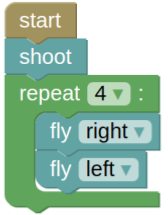
\includegraphics[width=.8\textwidth]{img/roboblocks-english}
\end{subfigure}
\begin{subfigure}{.62\textwidth}
{\lstset{numbers=none}
\begin{lstlisting}
highlightBlock(1);
shoot();
highlightBlock(2);
for (var i1_=0; i1_<4; i1_++) {
  highlightBlock(3);
  right();
  highlightBlock(4);
  left();
}
\end{lstlisting}}
\end{subfigure}
\caption{%
  Examples of a RoboJS (right) for a given RoboBlocks program (left). %
  Repeat loops require to generate unique names for iteration variables.
  Each original command is complemented by \texttt{highlightBlock(blockId)},
  so that the meta-interpreter knows which block to highlight.}
\label{fig:robojs-example}
\end{figure}

The generated JavaScript assumes to be executed within the context providing hooks
for actions (\texttt{fly}, \texttt{left}, \texttt{right}, \texttt{shoot}),
sensor functions (\texttt{color}, \texttt{position}),
and for meta-interpreting (\texttt{highlightBlock}).

We have not implemented a parser from RoboJS to RoboAST,
simply because we do not need this tranformation;
otherwise, there is no technical obstacle and the parser would be based on a similar PEG gramamar as for the RoboCode.


\subsection{Interpretation}
\label{sec:robomission-interpretation}

Instead of implementing our own interpreter of RoboCode,
we first transform the code through RoboAST into RoboJS
(described in section \ref{sec:robomission-robojs})
and then use JS-interpeter (REF) to run the code.
We could use any other interpreter that would satisfy the following
conditions:
\begin{enumerate}
\item is implemented in JavaScript (in order to run in the browser),
\item interprets a language that can be generated easily from the RoboAST
  (which includes most languages),
\item allows to define custom asynchronous hooks
  (needed for actions, sensors, and block highligting),
\item allows to step the code, or at least to impose a step or time limit
  (in order to break infinite loops).
\end{enumerate}
% TODO(opt): why not to use JS interpreter in browser: safety (sandbox requirement)
% + probably also not able to step the code or set the time limit, but I haven't verified this
There is nothing special about using JavaScript as the language being interpreted,
other that the JS-interpreter satisfies all our requirements
and is relatively simple to use.

The interpreter itself is a generator that yields actions, sensor requests and
meta-interpreting effects (block highlighting, checking for interruption).
The generator is wrapped into a saga
(see section \ref{sec:robomission-asynchronous-side-effects})
that handles all these asynchronous effects.
